\documentclass[aspectratio=169]{beamer}
\usetheme{Boadilla}
\usepackage[utf8]{inputenc}
\usepackage{ngerman}
\usepackage{url}
\usepackage{amsmath}
\usepackage{hyperref}
\usepackage{graphicx}
\usepackage{fontawesome}
\usepackage{irbookslide} %% remove this style file
\usepackage{newalg} %% remove this style file
\usepackage{pstricks,pst-node,pst-plot,pst-tree}

% Tikz based on a template by Aidan Hogan
\usepackage{tikz}
\usepackage{kg-macros}

\usepackage{listings}
\definecolor{mygreen}{rgb}{0,0.6,0}
\definecolor{mygray}{rgb}{0.5,0.5,0.5}
\definecolor{mymauve}{rgb}{0.58,0,0.82}
\lstset{ %
  backgroundcolor=\color{white},   % choose the background color
  basicstyle=\footnotesize,        % size of fonts used for the code
  breaklines=true,                 % automatic line breaking only at whitespace
  captionpos=b,                    % sets the caption-position to bottom
  commentstyle=\color{mygreen},    % comment style
  escapeinside={\%*}{*)},          % if you want to add LaTeX within your code
  frame=single,
  keywordstyle=\color{blue},       % keyword style
  stringstyle=\color{mymauve},     % string literal style
}


\begin{document}

\title[Levenshtein-Distanz]{Algorithmen zur Bestimmung der Levenshtein-Distanz von Zeichenketten (3./4. Semester) - \\ Natural Language Understanding (3/15)\\ 25 min.}   
\author[Dr. R. Usbeck]{Dr. Ricardo Usbeck\\\url{https://github.com/RicardoUsbeck/NLU}} 
\date{13.07.2020}

\begin{frame}
\titlepage
\end{frame}

\begin{frame}[fragile]\frametitle{Wiederholung 1/2: Dynamische Programmierung }
\begin{itemize}
    \item Datenstrukturen und effiziente Algorithmen II  (Bellman, 1957)
    \item Dynamische Programmierung ist eine Optimierungstechnik 
    %\item Perspektive: DP ist 'careful brute force' % exponentielle Probleme können manchmal in polynomieller Zeit gelöst werden. Es funktioniert aber nicht immer
    \pause
    \item Bekanntes Problem: Fibonacci(n) = Fibonacci(n-1) + Fibonacci(n-2) % mit F(k)=1 mit $k<=2, n>=1$
    \begin{itemize}
        \item Kann man exponentiell oder polynomiell implementieren % fibonacci ist goldener schnitt hoch n, % put Fibonaci number in dictionary, do not count recursions, constant time for call of n. you need to call n fibonacci numbers, the rest is stored
        \item Lösung: Bottum-Up, d.h. Teilprobleme speichern
    \end{itemize}
\end{itemize}
\begin{figure}
    \centering
    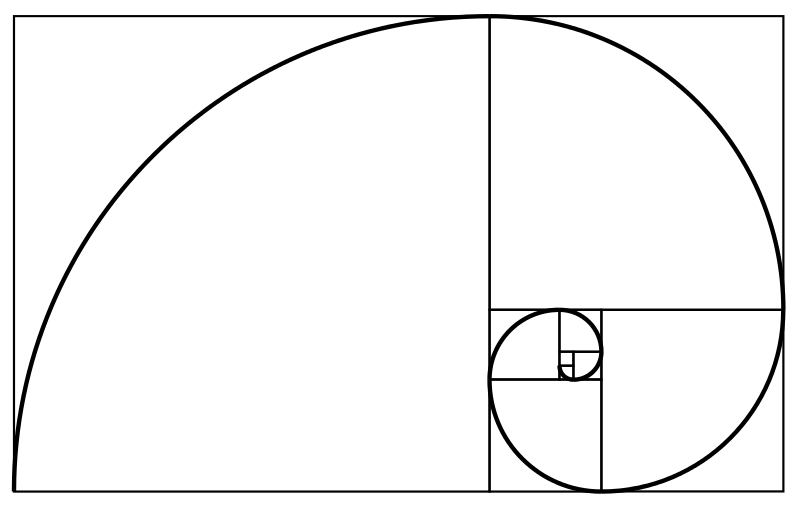
\includegraphics[width=0.4\linewidth]{800px-Fibonacci_spiral_34.svg.png}
\end{figure}
\end{frame}
 
\begin{frame}[fragile]\frametitle{Wiederholung 2/2: Dynamische Programmierung}

Dynamische Programmierung Schritte (Nach Cormen et al.):
\begin{enumerate}
    \item Charakterisiere Struktur der optimalen Lösung
    \item Definiere den Wert einer optimalen Lösung rekursiv
    \item Berechne den Wert der optimalen Lösung
    \item Wir konstruieren eine zugehörige optimale Teillösung aus bereits berechneten Daten            
\end{enumerate}
    \pause
Herangehensweisen für Probleme mit überlappenden aber unabhängigen Teilproblemen:
\begin{enumerate}
    \item Rekursive Berechnung (Brute-Force/nicht Dynamische Programmierung)% (Exakt das gleiche wie Memoized version, topologische Sortierung des Dependency DAG), hilft laufzeit abzulesen
    \item Memoization bei der rekursiven Variante hilft bei der Reduktion der Laufzeit %, runtime = number of subproblem * subproblem time
    \item Bottum-up Lösung des Problems durch Iteration aller optimalen Teilprobleme
    \item Möglichkeit zur Einsparung von Speicherplatz
\end{enumerate}

\end{frame}

\begin{frame} 
\frametitle{Motivation: Levenshtein-Distanz/Minimum-Edit-Distance}

\begin{itemize}
    \item Löst das String-Ähnlichkeitsproblem
    \pause
    \item Beispiele
    \begin{itemize}
        \item Rechtschreibkontrolle: graffe $\rightarrow$ graf, graft, grail, giraffe 
        \item Information Retrieval (z.B. Auto-Complete)  
        \item Natural Language Understanding (z.B. Kandidatensuche) 
        \item Machine Translation Systemen zum Finden von Alignments in parallelen Korpora 
        \item eHumanities zur Annotationsanalyse/Interrater Agreement Bestimmung 
        \item Nukleotidsequenzähnlichkeit (AATCCGCTAG $\rightarrow$ AAACCCTTAG)
    \end{itemize}
\end{itemize}
\end{frame}

\begin{frame}{Intuition: Levenshtein-Distanz/Minimum-Edit-Distance}
Definition der Operationen und ihrer Kosten um von String A zu String B zu kommen:
\begin{itemize}
    \item replace = 1, wenn Character i, j unterschiedlich sonst replace = 0
    \item delete = 1
    \item insert = 1
\end{itemize}
    \pause
\vspace{5mm}
Beispiel: Wieviele Operationen braucht man um von 'apfel' zu 'pferd' zu kommen? \pause
\begin{enumerate}
    \item Lösche 'a'
    \item Füge 'r' ein
    \item Ersetze 'l' durch 'd'
\end{enumerate}
\textcolor{blue}{$A=$apfel, $B=$pferd $edit_{A,B}(5,5) \Rightarrow 3$}
 \end{frame}
 
\begin{frame}{Intuition: Levenshtein-Distanz/Minimum-Edit-Distance}
\begin{itemize}
 
    \item Betrachte die beiden ersten Character und ignorieren erstmal den Substring, folgende Situation:
    \begin{enumerate}
        \item Characters sind gleich, tue nichts, kostet nichts (Antwort zum Teilproblem ist Antwort auf dieses Problem)
        \item Characters sind \textbf{nicht} gleich, entferne beide - replace, (Antwort zum Teilproblem ist Antwort auf dieses Problem)
        \item Characters sind \textbf{nicht} gleich, entferne von $A_i$ - delete (löst Teilproblem für A weiter)
        \item Characters sind \textbf{nicht} gleich, füge $B_i$ bei $A_i$ - insert (löst Teilproblem für B weiter)
    \end{enumerate}
    \pause
    \item (!) Wichtig, mit jedem Schritt bewegen wir uns weiter in einem der Teilprobleme 
   % \item Anzahl Teilprobleme: Betrachte für die Strings $A_{1,\dots,n}$ und $B_{1,\dots,m}$ alle Kombinationen von Substrings und finde Minimum-Edit-Distance $ = \Theta(|A|*|B|)$
\end{itemize}
\end{frame}



\begin{frame}{Definition: Levenshtein-Distanz/Minimum-Edit-Distance}
\begin{itemize}
    \item Gegeben zwei Strings: $A$ mit Länge $n$ und B mit Länge $m$ \pause
    \item Definiere $edit(i,j)$ als die Distanz zwischen $A_{1,\dots,i}$ und $B_{1,\dots,j}$ (erste $i$ / $j$ Zeichen)
    \item Definiere $edit(n,m)$ als Levenshtein-Distanz zwischen $A$ und $B$
    \pause
    %Basisfall
    \item $edit(0,j)=|j|$ und $edit(i,0)=|i|$
    \end{itemize}
    \pause

    \begin{equation}
        \begin{aligned}
        edit(i,j)=min( & \\
        & cost_{replace} + edit(i-1,j-1), \\
        & cost_{delete}+ edit(i-1,j), \\
        &  cost_{insert}+ edit(i,j-1)) \\
        \end{aligned}
    \end{equation}
    \pause
     In Worten: Minimale Anzahl an Operationen, um A nach B zu transformieren
%editdist(Aalpha, Bbeta) = min (editdist(alpha, beta)+2 oder edist(Aalpha,beta)+1 oder edit(alpha, Bbeta)+1)

\end{frame}


%\begin{frame}{Definition: Levenshtein-Distanz/Minimum-Edit-Distance}
%Beispiele:
%\begin{itemize}
%\item Levenshtein distance \emph{dog}-\emph{do}: 1
%\item Levenshtein distance \emph{cat}-\emph{cart}: 1
%\item Levenshtein distance \emph{cat}-\emph{cut}: 1
%\item Levenshtein distance \emph{cat}-\emph{act}: 2 % <- Dieser Faktor heißt Levenshtein Distanz
%\item Damerau-Levenshtein distance \emph{cat}-\emph{act}: 1
%\item Damerau-Levenshtein includes transposition as a fourth
%  possible operation.
%\end{itemize}
%\end{frame}


\begin{frame}[fragile]{Levenshtein-Distanz/Minimum-Edit-Distance (Rekursion)}
$edit(i,j)=min(cost_{replace} + edit(i-1,j-1),cost_{delete}+ edit(i-1,j), cost_{insert}+ edit(i,j-1), )$
\begin{lstlisting}[language=Python]
def edit(a,b):
    if len(a) == 0:
        return len(b)
    if len(b) == 0:
        return len(a)
    cost = 1 if a[-1]!= b[-1] else 0
    return min( edit(a[:-1],b[:-1]) + cost,
                edit(a,b[:-1]) +1,
                edit(a[:-1],b) +1)
\end{lstlisting}
\pause
 \begin{itemize}
     \item \url{https://colab.research.google.com/drive/1kZ7BP9OZ9Z2WSTcJrGGKcBpNLBXfWErt#scrollTo=gN78e6up20he&line=1&uniqifier=1}
 \end{itemize}
\end{frame}

\begin{frame}[fragile]{Levenshtein-Distanz/Minimum-Edit-Distance (Rekursion)}
$edit(i,j)=min(cost_{replace} + edit(i-1,j-1),cost_{delete}+ edit(i-1,j), cost_{insert}+ edit(i,j-1), )$
\begin{figure}
    \centering
    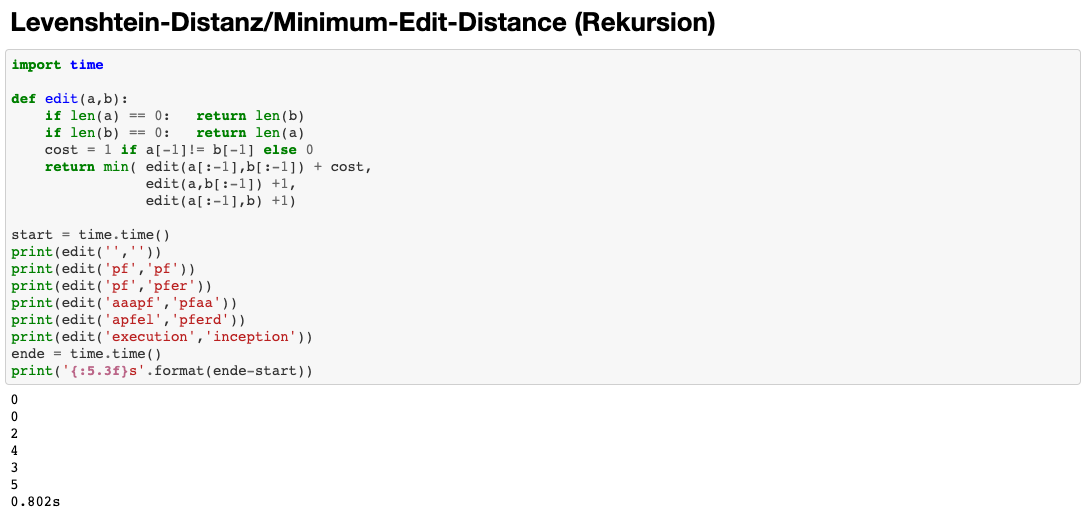
\includegraphics[width=0.9\linewidth]{code_recursion.png}
\end{figure}
\end{frame}

\begin{frame}[fragile]{Levenshtein-Distanz/Minimum-Edit-Distance (Rekursion)}
$edit(i,j)=min(cost_{replace} + edit(i-1,j-1),cost_{delete}+ edit(i-1,j), cost_{insert}+ edit(i,j-1), )$
\begin{lstlisting}[language=Python]
def edit(a,b):
    if len(a) == 0:
        return len(b)
    if len(b) == 0:
        return len(a)
    cost = 1 if a[-1]!= b[-1] else 0
    return min( edit(a[:-1],b[:-1]) + cost,
                edit(a,b[:-1]) +1,
                edit(a[:-1],b) +1)
\end{lstlisting}
 \begin{itemize}
     \item \url{https://colab.research.google.com/drive/1kZ7BP9OZ9Z2WSTcJrGGKcBpNLBXfWErt#scrollTo=gN78e6up20he&line=1&uniqifier=1}
     \item Laufzeit  $O(3^{n})$
     %\item Speicherbedarf $\Theta(1)$
 \end{itemize}
\end{frame}

\begin{frame}[fragile]{Levenshtein-Distanz/Minimum-Edit-Distance (Rekursion)}
Rekursionsbaum für $A=ab$ und $B=xy$ als Worst Case.\\
\scalebox{0.7}{
		\begin{tikzpicture}
    		\node[iri,anchor=center] (a) {edit(2,2)};  
    		\node[iri,anchor=center,below=1cm of a] (b) {edit(2,1)} edge[arrin]  (a);
    		        \node[iri,anchor=center,below=1cm of b] (b1) {edit(1,1)} edge[arrin]  (b);
    		            \node[iri,anchor=center,below=1cm of b1] (bb1) {edit(0,1)} edge[arrin]  (b1);
    		            \node[iri,anchor=center,left=4mm of bb1]  (bb2) {edit(1,0)} edge[arrin]  (b1);
    		            \node[iri,anchor=center,right=4mm of bb1] (bb3) {edit(0,0)} edge[arrin]  (b1);
    		        \node[iri,anchor=center,left=4mm of b1]  (b2) {edit(2,0)} edge[arrin]  (b);
    		        \node[iri,anchor=center,right=4mm of b1] (b3) {edit(1,0)} edge[arrin]  (b);
    		        
    		  \node[iri,anchor=center,left=4cm of b]  (c) {edit(1,2)} edge[arrin]  (a);
		            \node[iri,anchor=center,below=1cm of c] (c1) {edit(1,1)} edge[arrin]  (c);
        		    \node[iri,anchor=center,left=4mm of c1]  (c2) {edit(0,2)} edge[arrin]  (c);
    		            \node[iri,anchor=center,below=1cm of c1] (cc1) {edit(0,1)} edge[arrin]  (c1);
		                \node[iri,anchor=center,right=4mm of cc1] (cc3) {edit(0,0)} edge[arrin]  (c1);
		                \node[iri,anchor=center,left=4mm of cc1]  (cc2) {edit(1,0)} edge[arrin]  (c1);
    		        \node[iri,anchor=center,right=4mm of c1] (c3) {edit(0,1)} edge[arrin]  (c);
    		  
    		    \node[iri,anchor=center,right=4cm of b] (d) {edit(1,1)} edge[arrin]  (a);
    		          \node[iri,anchor=center,below=1cm of d] (dd) {edit(0,1)} edge[arrin]  (d);
    		          \node[iri,anchor=center,left=4mm of dd]  (dd2) {edit(1,0)} edge[arrin]  (d);
    		          \node[iri,anchor=center,right=4mm of dd] (dd3) {edit(0,0)} edge[arrin]  (d);
		\end{tikzpicture} }
\begin{itemize}
    \item Beobachtung: Raum aller möglichen Sequenzen ist sehr groß
    \item Lösung: Dynamische Programmierung über die Nutzung vorher berechneter, kleinere Teilprobleme von edit(i,j)!
\end{itemize}
\end{frame}

\begin{frame}[fragile]{Levenshtein-Distanz/Minimum-Edit-Distance}
$edit(0,j)=|j|$ und $edit(i,0)=|i|$\\
$edit(i,j)=min($\\
$cost_{replace} + edit(i-1,j-1),  $\\
$cost_{delete}+ edit(i-1,j),$\\
$cost_{insert}+ edit(i,j-1))  $\\
% Fragen, wo für steht eine Zelle (gleiches Beispiel)
\begin{table}[]
\begin{tabular}{|l|l|l|l|l|l|l|}
\hline
           & \textbf{} & \textbf{p} & \textbf{f} & \textbf{e} & \textbf{r} & \textbf{d} \\ \hline
\textbf{}  &           &            &            &            &            &            \\ \hline
\textbf{a} &           &            &            &            &            &            \\ \hline
\textbf{p} &           &            &            &            &            &            \\ \hline
\textbf{f} &           &            &            &            &            &            \\ \hline
\textbf{e} &           &            &            &            &            &            \\ \hline
\textbf{l} &           &            &            &            &            &            \\ \hline
\end{tabular}
\end{table}
\end{frame}


\begin{frame}[fragile]{Levenshtein-Distanz/Minimum-Edit-Distance}
$edit(0,j)=|j|$ und $edit(i,0)=|i|$\\
$edit(i,j)=min($\\
$cost_{replace} + edit(i-1,j-1),  $\\
$cost_{delete}+ edit(i-1,j),$\\
$cost_{insert}+ edit(i,j-1))  $\\
\begin{table}[]
\begin{tabular}{|l|l|l|l|l|l|l|}
\hline
           & \textbf{} & \textbf{p} & \textbf{f} & \textbf{e} & \textbf{r} & \textbf{d} \\ \hline
\textbf{}  & 0         & 1          & 2          & 3          & 4          & 5          \\ \hline
\textbf{a} & 1         &            &            &            &            &            \\ \hline
\textbf{p} & 2         &            &            &            &            &            \\ \hline
\textbf{f} & 3         &            &            &            &            &            \\ \hline
\textbf{e} & 4         &            &            &            &            &            \\ \hline
\textbf{l} & 5         &            &            &            &            &            \\ \hline
\end{tabular}
\end{table}
\end{frame}

\begin{frame}[fragile]{Levenshtein-Distanz/Minimum-Edit-Distance}
$edit(0,j)=|j|$ und $edit(i,0)=|i|$\\
$edit(i,j)=min($\\
$cost_{replace} + edit(i-1,j-1),  $\\
$cost_{delete}+ edit(i-1,j),$\\
$cost_{insert}+ edit(i,j-1))  $\\
\begin{table}[]
\begin{tabular}{|l|l|l|l|l|l|l|}
\hline
           & \textbf{} & \textbf{p} & \textbf{f} & \textbf{e} & \textbf{r} & \textbf{d} \\ \hline
\textbf{}  & 0         & 1          & 2          & 3          & 4          & 5          \\ \hline
\textbf{a} & 1         & 1          &            &            &            &            \\ \hline
\textbf{p} & 2         &            &            &            &            &            \\ \hline
\textbf{f} & 3         &            &            &            &            &            \\ \hline
\textbf{e} & 4         &            &            &            &            &            \\ \hline
\textbf{l} & 5         &            &            &            &            &            \\ \hline
\end{tabular}
\end{table}
\end{frame}

\begin{frame}[fragile]{Levenshtein-Distanz/Minimum-Edit-Distance}
$edit(0,j)=|j|$ und $edit(i,0)=|i|$\\
$edit(i,j)=min($\\
$cost_{replace} + edit(i-1,j-1),  $\\
$cost_{delete}+ edit(i-1,j),$\\
$cost_{insert}+ edit(i,j-1))  $\\
\begin{table}[]
\begin{tabular}{|l|l|l|l|l|l|l|}
\hline
           & \textbf{} & \textbf{p} & \textbf{f} & \textbf{e} & \textbf{r} & \textbf{d} \\ \hline
\textbf{}  & 0         & 1          & 2          & 3          & 4          & 5          \\ \hline
\textbf{a} & 1         & 1          & 2          &            &            &            \\ \hline
\textbf{p} & 2         &            &            &            &            &            \\ \hline
\textbf{f} & 3         &            &            &            &            &            \\ \hline
\textbf{e} & 4         &            &            &            &            &            \\ \hline
\textbf{l} & 5         &            &            &            &            &            \\ \hline
\end{tabular}
\end{table}
\end{frame}

\begin{frame}[fragile]{Levenshtein-Distanz/Minimum-Edit-Distance}
$edit(0,j)=|j|$ und $edit(i,0)=|i|$\\
$edit(i,j)=min($\\
$cost_{replace} + edit(i-1,j-1),  $\\
$cost_{delete}+ edit(i-1,j),$\\
$cost_{insert}+ edit(i,j-1))  $\\
\begin{table}[]
\begin{tabular}{|l|l|l|l|l|l|l|}
\hline
           & \textbf{} & \textbf{p} & \textbf{f} & \textbf{e} & \textbf{r} & \textbf{d} \\ \hline
\textbf{}  & 0         & 1          & 2          & 3          & 4          & 5          \\ \hline
\textbf{a} & 1         & 1          & 2          & 3          &            &            \\ \hline
\textbf{p} & 2         &            &            &            &            &            \\ \hline
\textbf{f} & 3         &            &            &            &            &            \\ \hline
\textbf{e} & 4         &            &            &            &            &            \\ \hline
\textbf{l} & 5         &            &            &            &            &            \\ \hline
\end{tabular}
\end{table}
\end{frame}


\begin{frame}[fragile]{Levenshtein-Distanz/Minimum-Edit-Distance}
$edit(0,j)=|j|$ und $edit(i,0)=|i|$\\
$edit(i,j)=min($\\
$cost_{replace} + edit(i-1,j-1),  $\\
$cost_{delete}+ edit(i-1,j),$\\
$cost_{insert}+ edit(i,j-1))  $\\
\begin{table}[]
\begin{tabular}{|l|l|l|l|l|l|l|}
\hline
           & \textbf{} & \textbf{p} & \textbf{f} & \textbf{e} & \textbf{r} & \textbf{d} \\ \hline
\textbf{}  & 0         & 1          & 2          & 3          & 4          & 5          \\ \hline
\textbf{a} & 1         & 1          & 2          & 3          & 4          &            \\ \hline
\textbf{p} & 2         &            &            &            &            &            \\ \hline
\textbf{f} & 3         &            &            &            &            &            \\ \hline
\textbf{e} & 4         &            &            &            &            &            \\ \hline
\textbf{l} & 5         &            &            &            &            &            \\ \hline
\end{tabular}
\end{table}
\end{frame}

\begin{frame}[fragile]{Levenshtein-Distanz/Minimum-Edit-Distance}
$edit(0,j)=|j|$ und $edit(i,0)=|i|$\\
$edit(i,j)=min($\\
$cost_{replace} + edit(i-1,j-1),  $\\
$cost_{delete}+ edit(i-1,j),$\\
$cost_{insert}+ edit(i,j-1))  $\\
\begin{table}[]
\begin{tabular}{|l|l|l|l|l|l|l|}
\hline
           & \textbf{} & \textbf{p} & \textbf{f} & \textbf{e} & \textbf{r} & \textbf{d} \\ \hline
\textbf{}  & 0         & 1          & 2          & 3          & 4          & 5          \\ \hline
\textbf{a} & 1         & 1          & 2          & 3          & 4          & 5          \\ \hline
\textbf{p} & 2         &            &            &            &            &            \\ \hline
\textbf{f} & 3         &            &            &            &            &            \\ \hline
\textbf{e} & 4         &            &            &            &            &            \\ \hline
\textbf{l} & 5         &            &            &            &            &            \\ \hline
\end{tabular}
\end{table}
\end{frame} 

\begin{frame}[fragile]{Levenshtein-Distanz/Minimum-Edit-Distance}
$edit(0,j)=|j|$ und $edit(i,0)=|i|$\\
$edit(i,j)=min($\\
$cost_{replace} + edit(i-1,j-1),  $\\
$cost_{delete}+ edit(i-1,j),$\\
$cost_{insert}+ edit(i,j-1))  $\\
\begin{table}[]
\begin{tabular}{|l|l|l|l|l|l|l|}
\hline
           & \textbf{} & \textbf{p} & \textbf{f} & \textbf{e} & \textbf{r} & \textbf{d} \\ \hline
\textbf{}  & 0         & 1          & 2          & 3          & 4          & 5          \\ \hline
\textbf{a} & 1         & 1          & 2          & 3          & 4          & 5          \\ \hline
\textbf{p} & 2         & 1          &            &            &            &            \\ \hline
\textbf{f} & 3         &            &            &            &            &            \\ \hline
\textbf{e} & 4         &            &            &            &            &            \\ \hline
\textbf{l} & 5         &            &            &            &            &            \\ \hline
\end{tabular}
\end{table}
\end{frame}

\begin{frame}[fragile]{Levenshtein-Distanz/Minimum-Edit-Distance}
$edit(0,j)=|j|$ und $edit(i,0)=|i|$\\
$edit(i,j)=min($\\
$cost_{replace} + edit(i-1,j-1),  $\\
$cost_{delete}+ edit(i-1,j),$\\
$cost_{insert}+ edit(i,j-1))  $\\
\begin{table}[]
\begin{tabular}{|l|l|l|l|l|l|l|}
\hline
           & \textbf{} & \textbf{p} & \textbf{f} & \textbf{e} & \textbf{r} & \textbf{d} \\ \hline
\textbf{}  & 0         & 1          & 2          & 3          & 4          & 5          \\ \hline
\textbf{a} & 1         & 1          & 2          & 3          & 4          & 5          \\ \hline
\textbf{p} & 2         & 1          & 2          & 3          & 4          & 5          \\ \hline
\textbf{f} & 3         &            &            &            &            &            \\ \hline
\textbf{e} & 4         &            &            &            &            &            \\ \hline
\textbf{l} & 5         &            &            &            &            &            \\ \hline
\end{tabular}
\end{table}
\end{frame}
 

\begin{frame}[fragile]{Levenshtein-Distanz/Minimum-Edit-Distance}
$edit(0,j)=|j|$ und $edit(i,0)=|i|$\\
$edit(i,j)=min($\\
$cost_{replace} + edit(i-1,j-1),  $\\
$cost_{delete}+ edit(i-1,j),$\\
$cost_{insert}+ edit(i,j-1))  $\\
\begin{table}[]
\begin{tabular}{|l|l|l|l|l|l|l|}
\hline
           & \textbf{} & \textbf{p} & \textbf{f} & \textbf{e} & \textbf{r} & \textbf{d} \\ \hline
\textbf{}  & 0         & 1          & 2          & 3          & 4          & 5          \\ \hline
\textbf{a} & 1         & 1          & 2          & 3          & 4          & 5          \\ \hline
\textbf{p} & 2         & 1          & 2          & 3          & 4          & 5          \\ \hline
\textbf{f} & 3         & 2          & 1          & 2          & 3          & 4          \\ \hline
\textbf{e} & 4         & 3          & 2          & 1          & 2          & 3          \\ \hline
\textbf{l} & 5         & 4          & 3          & 2          & 2          & 3          \\ \hline
\end{tabular}
\end{table}
\end{frame}

% Tabelle von Bücherei Typ zeigen mit Anzeige des kleinen Algorithms
% durchgehen, starten mti empty string comparisions (alles löschen, alles einfügen), diagonale steht für subproblem
% Fragen, wo für steht eine Zelle (gleiches Beispiel)
% schnell durchgehen, wenn der Buchstabe nicht passt
%%  zeige DP Tabelle von 8:28, frage: Was ist das für ein Zustand , wenn wir eine Tabelle haben A muss in B umgewandelt werden? Was bedeuted das? <- nach der einführung DP , beispiel und dann algorithmus


\begin{frame}{Levenshtein-Distanz/Minimum-Edit-Distance}
Bekannt als Wagner–Fischer-Algorithmus.
\begin{algorithm}{edit}{A,B}
\begin{FOR}
{i \= 0 \TO |A|}
m[i,0] = i
\end{FOR}\\
\begin{FOR}
{j \= 0 \TO |B|}
m[0,j] = j
\end{FOR}\\
\begin{FOR}
{i \= 1 \TO |A|}
\begin{FOR}
{j \= 1 \TO |B|}
\begin{IF}{A[i]=B[j]}
m[i,j] = \min\{m[i\mbox{-}1, j] \mbox{+} 1,m[i, j\mbox{-}1] \mbox{+} 1,m[i\mbox{-}1,j\mbox{-}1] \}
\ELSE
m[i,j] = \min\{m[i\mbox{-}1, j] \mbox{+} 1,m[i, j\mbox{-}1] \mbox{+} 1,m[i\mbox{-}1,j\mbox{-}1]\mbox{+}1 \}
\end{IF}
\end{FOR}
\end{FOR}\\
\RETURN{m[|A|,|B|]}
\end{algorithm}
Operations: insert (cost 1), delete (cost 1), replace (cost 1), copy (cost 0)
\end{frame}

\begin{frame}{Levenshtein-Distanz/Minimum-Edit-Distance}
\begin{algorithm}{edit}{A,B}
\begin{FOR}
{i \= 0 \TO |A|}
m[i,0] = i
\end{FOR}\\
\begin{FOR}
{j \= 0 \TO |B|}
m[0,j] = j
\end{FOR}\\
\begin{FOR}
{i \= 1 \TO |A|}
\begin{FOR}
{j \= 1 \TO |B|}
\begin{IF}{A[i]=B[j]}
m[i,j] = \min\{m[i\mbox{-}1, j] \mbox{+} 1, \myred{m[i, j\mbox{-}1] \mbox{+} 1},m[i\mbox{-}1,j\mbox{-}1] \}
\ELSE
m[i,j] = \min\{m[i\mbox{-}1, j] \mbox{+} 1, \myred{m[i, j\mbox{-}1] \mbox{+} 1},m[i\mbox{-}1,j\mbox{-}1]\mbox{+}1 \}
\end{IF}
\end{FOR}
\end{FOR}\\
\RETURN{m[|A|,|B|]}
\end{algorithm}
Operations: \myred{insert (cost 1)}, delete (cost 1), replace (cost1), copy (cost 0)
\end{frame}

\begin{frame}{Levenshtein-Distanz/Minimum-Edit-Distance}
\begin{algorithm}{edit}{A,B}
\begin{FOR}
{i \= 0 \TO |A|}
m[i,0] = i
\end{FOR}\\
\begin{FOR}
{j \= 0 \TO |B|}
m[0,j] = j
\end{FOR}\\
\begin{FOR}
{i \= 1 \TO |A|}
\begin{FOR}
{j \= 1 \TO |B|}
\begin{IF}{A[i]=B[j]}
m[i,j] = \min\{ \myred{m[i\mbox{-}1, j] \mbox{+} 1},m[i, j\mbox{-}1] \mbox{+} 1,m[i\mbox{-}1,j\mbox{-}1] \}
\ELSE
m[i,j] = \min\{ \myred{m[i\mbox{-}1, j] \mbox{+} 1},m[i, j\mbox{-}1] \mbox{+} 1,m[i\mbox{-}1,j\mbox{-}1]\mbox{+}1 \}
\end{IF}
\end{FOR}
\end{FOR}\\
\RETURN{m[|A|,|B|]}
\end{algorithm}
Operations: insert (cost 1), \myred{delete (cost 1)}, replace (cost 1), copy (cost 0)
\end{frame}

\begin{frame}{Levenshtein-Distanz/Minimum-Edit-Distance}
\begin{algorithm}{edit}{A,B}
\begin{FOR}
{i \= 0 \TO |A|}
m[i,0] = i
\end{FOR}\\
\begin{FOR}
{j \= 0 \TO |B|}
m[0,j] = j
\end{FOR}\\
\begin{FOR}
{i \= 1 \TO |A|}
\begin{FOR}
{j \= 1 \TO |B|}
\begin{IF}{A[i]=B[j]}
m[i,j] = \min\{m[i\mbox{-}1, j] \mbox{+} 1,m[i, j\mbox{-}1] \mbox{+} 1,m[i\mbox{-}1,j\mbox{-}1] \}
\ELSE
m[i,j] = \min\{m[i\mbox{-}1, j] \mbox{+} 1,m[i, j\mbox{-}1] \mbox{+} 1, \myred{m[i\mbox{-}1,j\mbox{-}1]\mbox{+}1} \}
\end{IF}
\end{FOR}
\end{FOR}\\
\RETURN{m[|A|,|B|]}
\end{algorithm}
Operations: insert (cost 1), delete (cost 1), \myred{replace (cost 1)}, copy (cost 0)
\end{frame}

\begin{frame}{Levenshtein-Distanz/Minimum-Edit-Distance}
\begin{algorithm}{edit}{A,B}
\begin{FOR}
{i \= 0 \TO |A|}
m[i,0] = i
\end{FOR}\\
\begin{FOR}
{j \= 0 \TO |B|}
m[0,j] = j
\end{FOR}\\
\begin{FOR}
{i \= 1 \TO |A|}
\begin{FOR}
{j \= 1 \TO |B|}
\begin{IF}{A[i]=B[j]}
m[i,j] = \min\{m[i\mbox{-}1, j] \mbox{+} 1,m[i, j\mbox{-}1] \mbox{+} 1, \myred{m[i\mbox{-}1,j\mbox{-}1]} \}
\ELSE
m[i,j] = \min\{m[i\mbox{-}1, j] \mbox{+} 1,m[i, j\mbox{-}1] \mbox{+} 1,m[i\mbox{-}1,j\mbox{-}1]\mbox{+}1 \}
\end{IF}
\end{FOR}
\end{FOR}\\
\RETURN{m[|A|,|B|]}
\end{algorithm}
Operations: insert (cost 1), delete (cost 1), replace (cost 1), \myred{copy (cost 0)}
\end{frame}


\begin{frame}[fragile]{Levenshtein-Distanz/Minimum-Edit-Distance}
\begin{lstlisting}[language=Python]
def edit(a,b):
    if len(a) < len(b): return edit(b, a)
    a = ' ' + a
    b = ' ' + b
    d = {}
    S, T = len(a), len(b)
    for i in range(S):
        d[i, 0] = i
    for j in range (T):
        d[0, j] = j
    for j in range(1,T):
        for i in range(1,S):
            if a[i] == b[j]:
                d[i, j] = d[i-1, j-1]
            else:
                d[i, j] = min(d[i-1, j], d[i, j-1], d[i-1, j-1]) + 1
    return d[S-1, T-1]
\end{lstlisting}
\end{frame}

\begin{frame}[fragile]{Levenshtein-Distanz/Minimum-Edit-Distance}
 \begin{itemize}
    \item Speicherbedarf $O(|a|\cdot|b|)$
    \item Laufzeit $O(|a|\cdot|b|)$
    \item \url{https://colab.research.google.com/drive/1kZ7BP9OZ9Z2WSTcJrGGKcBpNLBXfWErt#scrollTo=3_2B4Lin226_&line=2&uniqifier=1}
\end{itemize}
\end{frame}

\begin{frame}[fragile]{Levenshtein-Distanz/Minimum-Edit-Distance}
\begin{figure}
    \centering
    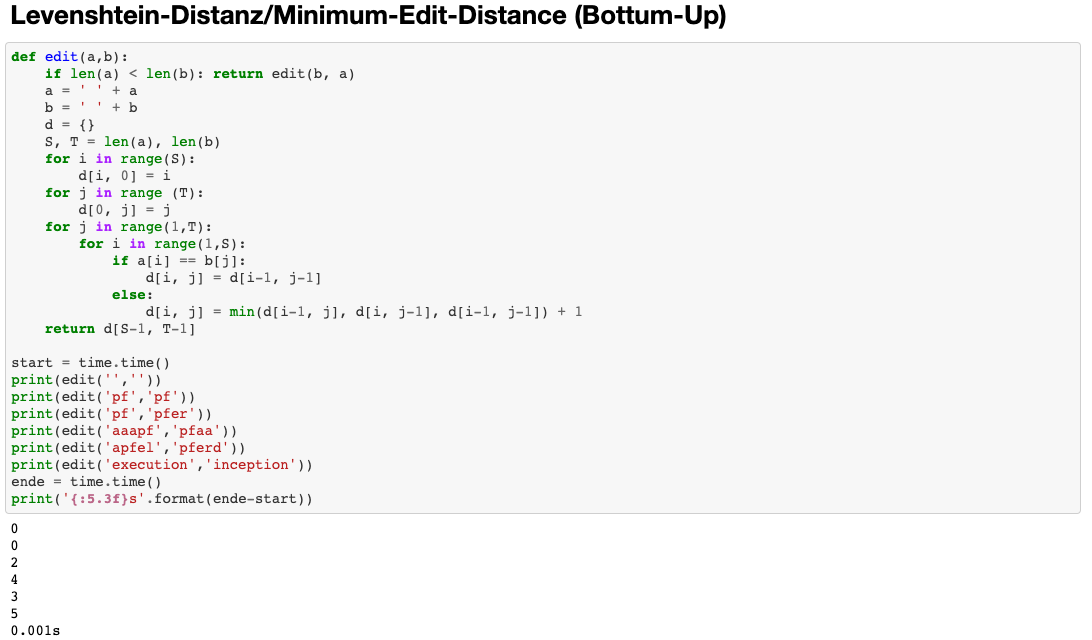
\includegraphics[width=0.85\linewidth]{code_bottom_up.png}
\end{figure}
\end{frame}

\begin{frame}[fragile]{Levenshtein-Distanz/Minimum-Edit-Distance (Speicher reduzieren)}
\begin{lstlisting}[language=Python]
def edit(a, b):
  if len(a) < len(b): return edit(b, a)
  if len(a) == 0:     return len(b)
  if len(b) == 0:     return len(a)
  v0, v1 = [None] * (len(a) + 1) ,  [None] * (len(a) + 1)
  for i in range(len(v0)):
      v0[i] = i
  for i in range(len(a)):
      v1[0] = i + 1
      for j in range(len(b)):
          cost = 0 if a[i] == b[j] else 1
          v1[j + 1] = min(v1[j] + 1, v0[j + 1] + 1, v0[j] + cost)
      for j in range(len(v0)):
          v0[j] = v1[j]

  return v1[len(b)]
\end{lstlisting}
\end{frame}

\begin{frame}[fragile]{Levenshtein-Distanz/Minimum-Edit-Distance (Speicher reduzieren)}
\begin{itemize}
    \item Speicherbedarf $O(min(|a|,|b|))$
    \item Laufzeit $O(|a|\cdot|b|)$
    \item \url{https://colab.research.google.com/drive/1kZ7BP9OZ9Z2WSTcJrGGKcBpNLBXfWErt#scrollTo=4AX2m6pk4EwO&line=1&uniqifier=1}
\end{itemize}
\end{frame}

\begin{frame}[fragile]{Levenshtein-Distanz/Minimum-Edit-Distance (Speicher reduzieren)}
\begin{figure}
    \centering
    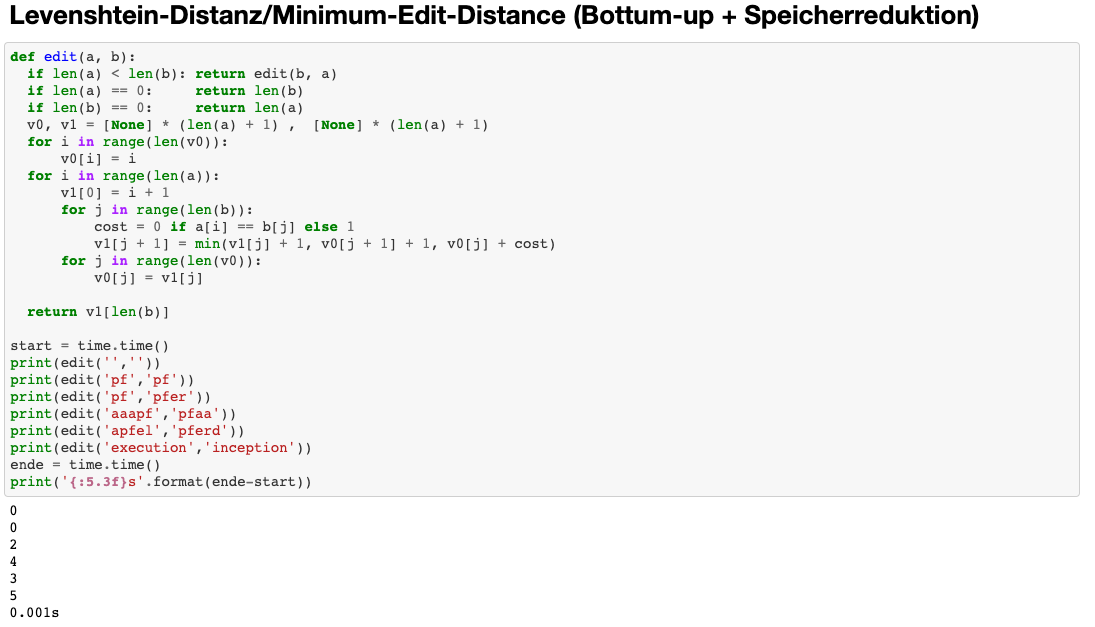
\includegraphics[width=0.9\linewidth]{code_bottom_up_space.png}
\end{figure}
\end{frame}





%% HAMMING DISTANZ
% number of substitutions
% Selbstlernen Schreiben Sie einen korrekten Algorithmus für die HAMMING Distanz
% Selbstlernen Beweisen sie dass, editDistanz <= hammingditanz?
% Selbstlernen     %%Hinzufügen
    %\item LowerBound $edit(X,Y)>= ||X|-|Y||$ für unterschiedlich lange String
    %\item UpperBound $edit(X,Y)>= 2 * max (|X|,|Y|)$
% Selbstlernen Bauen Sie den Code so um, dass bei der rekursiven Variante die Anzahl der Calls mitgeloggt und auf die KOmmandaozeile geschrieben wird
% Selbstlernen  Wenn man die kosten für replace unendlich groß macht, löst man das longest common subsequence probelm
% Selbstlernen  What are the Levenshtein editing operations that transform \emph{cat} into \emph{catcat}?
% Selbstlernen If we are only interested in the distance if it is smaller than a threshold k, then it suffices to compute a diagonal stripe of width 2k+1 in the matrix. In this way, the algorithm can be run in O(kl) time, where l is the length of the shortest string.[2]
% Selbstlernen We can give different penalty costs to insertion, deletion and substitution. We can also give penalty costs that depend on which characters are inserted, deleted or substituted.
% Selbstlernen This algorithm parallelizes poorly, due to a large number of data dependencies. However, all the cost values can be computed in parallel, and the algorithm can be adapted to perform the minimum function in phases to eliminate dependencies.
% Selbstlernen By examining diagonals instead of rows, and by using lazy evaluation, we can find the Levenshtein distance in O(m (1 + d)) time (where d is the Levenshtein distance), which is much faster than the regular dynamic programming algorithm if the distance is small.[3]


\begin{frame}{Take-Away und Ausblick} 
Was haben wir gelernt?
\begin{itemize}
    \item Levenshtein-Distanz in Theorie und Praxis
\end{itemize}
Ist das jetzt sinnvoll?
\begin{itemize}
    \item Immer noch industrierelevant: Bspw. Elastic Search, Chatbots, Autocomplete
    \item Inspiration für neue DL-Architekturen: Gu, J., Wang, C., and Zhao, J. (2019). Levenshtein transformer. In Advances in Neural Information Processing Systems (pp. 11181-11191), \url{http://papers.nips.cc/paper/9297-levenshtein-transformer.pdf}
\end{itemize}
Wo können wir weiter üben?
\begin{itemize}
    \item \url{http://github.com/RicardoUsbeck/NLU}
\end{itemize}
Was passiert beim nächsten Mal?
\begin{itemize}
    \item Memoization, Gewichtete Levenshtein-Distanz
    \item Language Modeling mit N-Grams
    \item Schnelle Rechtschreibkorrektur
\end{itemize}
\end{frame}



%%%% REFERENZEN %%%%
\begin{frame}\frametitle{Quellen}
\begin{itemize}
    \item Cormen, T. H., Leiserson, C. E., Rivest, R., and Stein, C. (2017). Algorithmen-Eine Einführung. Walter de Gruyter GmbH and Co KG.
    \item Jurasky, D., and Martin, J. H. (2000). Speech and Language Processing: An introduction to natural language Processing. Computational Linguistics and Speech Recognition. Prentice Hall, New Jersey. (\url{https://web.stanford.edu/~jurafsky/slp3/2.pdf})
    \item Levenshtein, V. I. (1966, February). Binary codes capable of correcting deletions, insertions, and reversals. In Soviet physics doklady (Vol. 10, No. 8, pp. 707-710).
    \item Wagner, R. A., and Fischer, M. J. (1974). The string-to-string correction problem. Journal of the ACM (JACM), 21(1), 168-173. (\url{https://dl.acm.org/doi/pdf/10.1145/321796.321811})
    \item Fred J. Damerau: A technique for computer detection and correction of spelling errors. In: Communications of the ACM. Band 7, Nr. 3, März 1964, S. 171–176.
    \item \url{http://www.let.rug.nl/kleiweg/lev/}, 24.06.2020, Online Tool
    \item \url{https://en.wikibooks.org/wiki/Algorithm_Implementation/Strings/Levenshtein_distance\#Python}, 21.06.2020 
    % https://lmb.informatik.uni-freiburg.de/lectures/AlgoDatESE/ws1314/Vorlesung_AlgoDatESE+IEMS_14.pdf nicht benutzt
\end{itemize}
\end{frame}

\begin{frame}\frametitle{Lernvideos/Blended Learning}
\begin{itemize}
    \item \url{https://www.youtube.com/watch?v=HXNhEYqFo0o}, 14.06.2020
    \item \url{https://www.youtube.com/watch?v=MiqoA-yF-0M}, 19.06.2020 
    \item \url{https://www.youtube.com/watch?v=OQ5jsbhAv_M}, 19.06.2020
    \item \url{https://www.youtube.com/watch?v=Xxx0b7djCrs}, 19.06.2020
    \item \url{https://www.youtube.com/watch?v=ocZMDMZwhCY}, 19.06.2020
    \item \url{https://www.youtube.com/watch?v=8Q2IEIY2pDU}, 21.06.2020
    \item \url{https://www.youtube.com/watch?v=qp8YwtvS3Uo}, 21.06.2020
    \item \url{https://www.youtube.com/watch?v=xFd5P9nyhTw}, 30.06.2020
\end{itemize}
\end{frame}


\begin{frame}{\textbf{Danke für Ihre Aufmerksamkeit!}}
    \begin{center}
        \small{\faGraduationCap \hspace{0.15em} {Lernmaterial (VL, Selbsttests, Übungen, Links zu Jupyter Notebooks...)\\\small{\faGithub \hspace{0.15em} {\href{https://github.com/RicardoUsbeck/NLU}{http://github.com/RicardoUsbeck/NLU}}}}} \\
        \smallskip
        \Huge {Welche Fragen haben Sie?} \\
        
    \end{center}
    \begin{columns}
	\column{.59\textwidth}
	\tiny
	\begin{itemize}
	    \item Wladimir Iossifowitsch Lewenstein war ein russischer Mathematiker, der durch die nach ihm benannte, 1965 erfundene Levenshtein-Distanz bekannt wurde. Er machte 1958 seinen Abschluss an der Lomonossow-Universität und lehrte und forschte anschließend am Moskauer Keldysch-Institut für angewandte Mathematik - Wikipedia. Annectode: Dynamische Programmierung wurde durch Bellman vorgeschlagen, da Dynamic Optimization zu sehr nach Forschung klang.
	\end{itemize}
	\column{.4\textwidth}
	\centering
	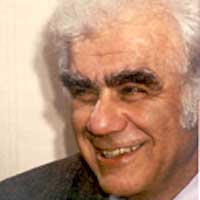
\includegraphics[width=40px,keepaspectratio]{vladimir_levenshtein.jpg}\\
	\tiny \textcolor{gray}{Quelle: \url{https://www.computerhope.com/people/vladimir_levenshtein.htm}}

\end{columns}
\end{frame}
 
\begin{frame}{Gewichtete Levenshtein-Distanz}
\begin{itemize}
\item Passe die Kosten pro Operation basierend auf den jeweiligen Characterpaar an
\item Wurde entwickelt um Tippfehler zu korrigieren, bspw. \emph{m} ist wahrscheinlich mit \emph{n} verwechselt als mit \emph{q}
\item Darum kann man die Edit-Distanz von \emph{m} nach \emph{n} kleiner machen als \emph{q}
\item Dazu braucht man eine Gewichtmatrix!
\item Anwendung: Computational Biology - Zwei Nukleotidsequenzen alignen (AGTC vs AGGT)
    \begin{itemize}
        \item DNA Transformation
        \item C$\rightarrow$G niedriges Gewicht, weil wahrscheinlicher als  C$\rightarrow$A
    \end{itemize} 
\item Anwendung: Cultural Analytics - Annotations Analyse/Interrater Agreement %https://elib.uni-stuttgart.de/bitstream/11682/10901/1/special-issue.pdf
\end{itemize}
\end{frame}

\end{document}
